% https://tex.stackexchange.com/a/172847/173708
\documentclass[tikz,border=5]{standalone}

\usepackage{xcolor}
\usepackage{tikz}
\usepackage{pgfplots}

\newlength{\xdim}

\definecolor{findOptimalPartition}{HTML}{D7191C}
\definecolor{storeClusterComponent}{HTML}{FDAE61}
\definecolor{dbscan}{HTML}{ABDDA4}
\definecolor{constructCluster}{HTML}{2B83BA}

\begin{document}
%\begin{figure}
%\centering
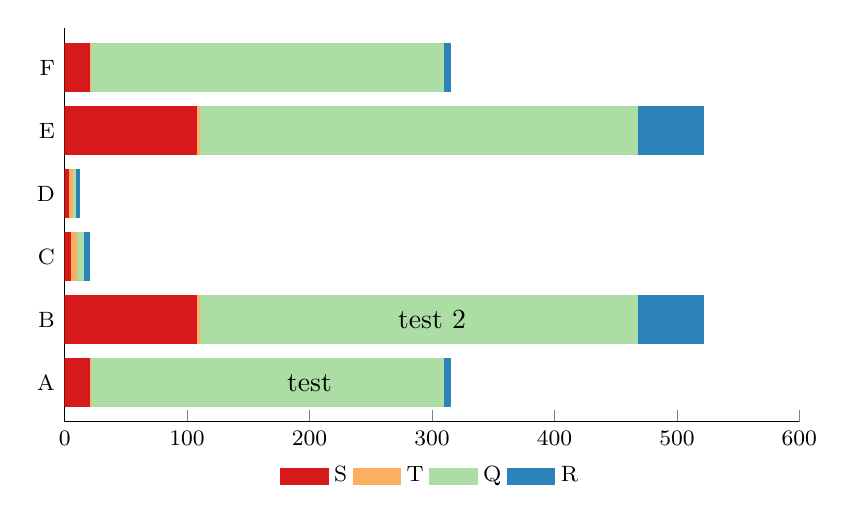
\begin{tikzpicture}
\begin{axis}[
    xbar stacked,
    legend style={
    legend columns=4,
        at={(xticklabel cs:0.5)},
        anchor=north,
        draw=none
    },
    ytick=data,
    axis y line*=none,
    axis x line*=bottom,
    tick label style={font=\footnotesize},
    legend style={font=\footnotesize},
    label style={font=\footnotesize},
    xtick={0,100,200,300,400,500,600},
    width=.9\textwidth,
    bar width=6mm,
    xlabel={Time in ms},
    yticklabels={A, B, C, D, E, F},
    xmin=0,
    xmax=600,
    area legend,
    y=8mm,
    enlarge y limits={abs=0.625},
]
\addplot[findOptimalPartition,fill=findOptimalPartition] coordinates
{(20,0) (108,1) (5,2) (3,3) (108,4) (20,5)};
\addplot[storeClusterComponent,fill=storeClusterComponent] coordinates
{(1.4,0) (2,1) (5,2) (3,3) (2,4) (1,5)};
\addplot[dbscan,fill=dbscan] coordinates
{(288,0) (358,1) (5,2) (3,3) (358,4) (288,5)};
\addplot[constructCluster,fill=constructCluster] coordinates
{(6,0) (54,1) (5,2) (3,3) (54,4) (6,5)};
\legend{S, T, Q, R}
\coordinate (A) at (200,0);% ******** start of changes ************
\coordinate (B) at (300,8mm);
\end{axis}  
\node at (A) {test};
\node at (B) {test 2};% ********* end of changes **********
\end{tikzpicture}
%\caption{X}
%\label{fig:stats}
%\end{figure}
\end{document}